\documentclass[11pt,a4paper]{report}

% Packages and commands file
\usepackage[utf8]{inputenc}
\usepackage[T1]{fontenc}
\usepackage[english]{babel}
\usepackage{amsmath}
\usepackage{ae}
\usepackage{icomma}
\usepackage{units}
\usepackage{color}
\usepackage{graphicx}
\usepackage{epstopdf}
\usepackage{subfigure}
\usepackage{bbm}
\usepackage{caption}
\usepackage{natbib}
\usepackage{multirow}
\usepackage{array}
\usepackage{geometry}
\usepackage{fancyhdr}
\usepackage{fncychap}
\usepackage[hyphens]{url}
\usepackage[breaklinks,pdfpagelabels=false]{hyperref}
\usepackage{lettrine}
\usepackage{eso-pic}

\newcommand{\rd}{\ensuremath{\mathrm{d}}}
\newcommand{\id}{\ensuremath{\,\rd}}
\newcommand{\degC}{\ensuremath{\,\unit{^\circ C}}}

% Fancyheader shortcuts
\newcommand{\setdefaulthdr}{%
\fancyhead[L]{\slshape \rightmark}%
\fancyhead[R]{\slshape \leftmark}%
\fancyfoot[C]{\thepage}%
}
\newcommand{\setspecialhdr}{%
\fancyhead[L]{ }%
\fancyhead[R]{\slshape \leftmark}%
\fancyfoot[C]{\thepage}%
}

\newcommand{\mail}[1]{\href{mailto:#1}{\nolinkurl{#1}}}
\newcommand{\backgroundpic}[3]{%
	\put(#1,#2){
		\parbox[b][\paperheight]{\paperwidth}{%
			\centering
			\includegraphics[width=\paperwidth,height=\paperheight,keepaspectratio]{#3}
			\vfill
}}}




\graphicspath{{./include/images/}}

% Settings (Metadata)
% References, choose bst-file
\bibliographystyle{plainnat}

% PDF Metadata and link styles
\hypersetup{
		pdftitle={Master's Thesis: },%
		pdfauthor={Erik Brännström},%
    colorlinks=true,%
    citecolor=black,%
    filecolor=black,%
    linkcolor=black,%
    urlcolor=black
}

% Dropping initial letter color
\renewcommand{\LettrineFontHook}{\color[gray]{0.5}}

% Chapter headings style (fncychap)
\makeatletter
\ChNumVar{} % sets the style for digit
\ChTitleVar{\Huge\bfseries\centering} % sets the style for title
\ChRuleWidth{4pt} % Set RW=4pt
\ChNameUpperCase % Make name uppercase
\renewcommand{\DOCH}{
\centering
{\CNoV {\fontsize{60pt}{20pt}\selectfont\thechapter} }
\vskip 40\p@}
\renewcommand{\DOTI}[1]{%
\CTV\FmTi{#1}\par\nobreak
\vskip 40\p@}
\renewcommand{\DOTIS}[1]{%
\CTV\FmTi{#1}\par\nobreak
\vskip 40\p@}
\makeatother

% Single page abstract
\renewenvironment{abstract}%
{\begin{center} \bfseries \abstractname \end{center}}%
{\vspace{2\baselineskip}}%

% Figure & Table captions
\captionsetup{margin=10pt,font=small,labelfont=bf}
\captionsetup[table]{position=top}
\setlength{\extrarowheight}{4pt}
\addtolength{\headheight}{\baselineskip}

% Fancyheader (see packagescommands.tex for default/special)
\pagestyle{fancy}
\setdefaulthdr

% Stolen settings (unknown origin):
% Alter some LaTeX defaults for better treatment of figures:
% See p.105 of "TeX Unbound" for suggested values.
% See pp. 199-200 of Lamport's "LaTeX" book for details.
%   General parameters, for ALL pages:
\renewcommand{\topfraction}{0.9}	% max fraction of floats at top
\renewcommand{\bottomfraction}{0.8}	% max fraction of floats at bottom
%   Parameters for TEXT pages (not float pages):
\setcounter{topnumber}{2}
\setcounter{bottomnumber}{2}
\setcounter{totalnumber}{4}     % 2 may work better
\setcounter{dbltopnumber}{2}    % for 2-column pages
\renewcommand{\dbltopfraction}{0.9}	% fit big float above 2-col. text
\renewcommand{\textfraction}{0.07}	% allow minimal text w. figs
%   Parameters for FLOAT pages (not text pages):
\renewcommand{\floatpagefraction}{0.7}	% require fuller float pages
% N.B.: floatpagefraction MUST be less than topfraction !!
\renewcommand{\dblfloatpagefraction}{0.7}	% require fuller float pages

% remember to use [htp] or [htpb] for placement

\begin{document}

% Title page and abstract
% Chalmers title page
\begin{titlepage}

\AddToShipoutPicture{\backgroundpic{-4}{56.7}{./include/images/frontpage}}
\mbox{}
\vfill
\addtolength{\voffset}{2cm}
\begin{flushleft}
	{\noindent {\Huge Automated analysis and planning of social network marketing} \\[0.5cm]
	\emph{\Large Master's Thesis in Software Engineering} \\[.8cm]

	{\huge ERIK BRÄNNSTRÖM}\\[.8cm]

	{\Large Division of Software Engineering \\
	\textsc{Chalmers University of Technology} \\
	Göteborg, Sweden 2012 \\
	Master's Thesis 2012:X\\
	}
	}
\end{flushleft}

\end{titlepage}
\ClearShipoutPicture
% End Chalmers title page

\pagestyle{empty}
\newpage
\clearpage
\mbox{}
\newpage
\clearpage
\thispagestyle{empty}

\onecolumn
\begin{abstract}
Lorem ipsum dolor sit amet, consectetur adipisicing elit, sed do eiusmod tempor incididunt ut labore et dolore magna aliqua. Ut enim ad minim veniam, quis nostrud exercitation ullamco laboris nisi ut aliquip ex ea commodo consequat. Duis aute irure dolor in reprehenderit in voluptate velit esse cillum dolore eu fugiat nulla pariatur. Excepteur sint occaecat cupidatat non proident, sunt in culpa qui officia deserunt mollit anim id est laborum.
\end{abstract}

\newpage
\clearpage
\mbox{}
\newpage
\clearpage
\thispagestyle{empty}
\section*{Acknowledgements}
Lorem ipsum dolor sit amet, consectetur adipisicing elit, sed do eiusmod tempor incididunt ut labore et dolore magna aliqua. Ut enim ad minim veniam, quis nostrud exercitation ullamco laboris nisi ut aliquip ex ea commodo consequat. Duis aute irure dolor in reprehenderit in voluptate velit esse cillum dolore eu fugiat nulla pariatur. Excepteur sint occaecat cupidatat non proident, sunt in culpa qui officia deserunt mollit anim id est laborum. \\[1cm]

\hfill The Authors, Location 11/9/11
\newpage
\clearpage
\mbox{}

% Table of contents
\newpage
\pagenumbering{roman}
\setcounter{page}{1}
\pagestyle{fancy}
\setspecialhdr
\tableofcontents

% Main area
\newpage
\setdefaulthdr
\pagenumbering{arabic}
\setcounter{page}{1}

\chapter{Introduction}
As more and more people are using the Internet on a daily basis, the area of online marketing is expanding as a way for organizations to reach large audiences for a relatively small amount of money. A site that displays advertisement, the publisher, is often paid by the advertiser based on the number of times visitors see or click on the ads, but it may also be coupled with other requirements, such as that the visitor goes on to buy a product from the advertiser in a given time span. Because advertisers want to pay as little as possible while still getting good results and distributors often preferring to only show relevant information to their visitors to keep them coming back, the advertisement is typically tailored to the expected interests of the visiting user.

The material is created by the advertiser, its impact analyzed and based on these results, material is created, adapted or removed from circulation to better suit a new or existing target audience. This circular process requires a lot of manual labor since the analysis results must be understood and applied to the context of the material as well as the target group. There is a lot of data that needs to be correlated, a task that is well suited for computers.

On Duego, a social networking company founded in 2010, online advertisement is leveraged as a way to promote the site to new users. The process of managing the online marketing data follows the manual process described above. The goal of Duego and this thesis is to automate parts of this process using a software solution.

The system is required to analyze existing campaigns with regard to ads and target groups along with campaign metrics, for example the number of times an ad is shown. This data is then used as a basis for suggesting new ads. The data set that will be used in production consists of hundreds of different campaigns, each with a large number of ads. Along with the attributes of both campaigns and ads, this means that the complete advertisement data set consists of hundreds of thousands of possible attribute combinations that need to be analyzed.

A generalization of this problem is knowledge discovery in databases (KDD) and, more specifically, data mining. Data mining is the process of delegating and automating the task of identifying knowledge that by some definition is useful in a large set of data to a computer, either fully or partially.

The research question for this thesis is how to use historical online marketing data to automate the creation of new advertisement campaigns. The answer to this question is presented as a procedure that is applicable to online advertisers. The following subsections will describe terminology from the fields of automation and marketing respectively. This is followed by a description of the problem this thesis addresses and finally a limitation of the scope of this paper.

\section{Automation}
\begin{figure}[htb] \centering 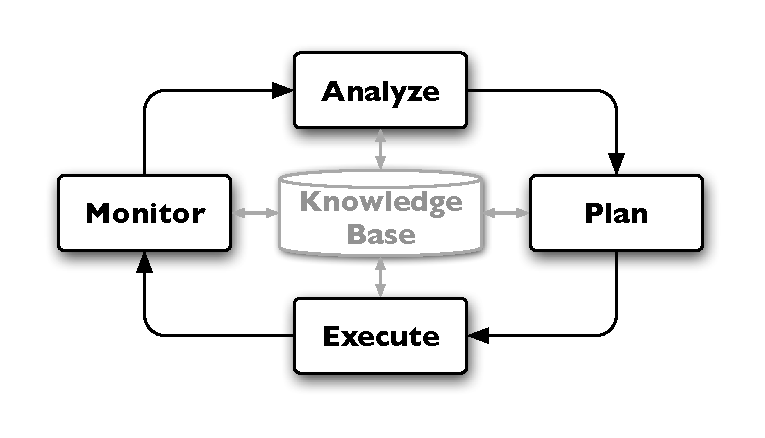
\includegraphics[width=0.5\textwidth]{mape.eps}
	\caption{General MAPE control loop}
	\label{fig:MAPE}
\end{figure}

Useful terminology is defined by \citet{IBM2006} in the field of autonomic computing. Figure \ref{fig:MAPE} shows an autonomic manager, which is a component that collects data from a system and, based on this data, performs actions with the purpose of improving the system. This control loop is divided into four subtasks called monitor (collect system information), analyze (correlate and model data), plan (design behavior required to reach goal) and execute (run the planned actions), sometimes referred to as MAPE. Each subtask can optionally interact with a knowledge base for storing and retrieving data. This will then be applied to online marketing.

\section{Marketing}
A number of marketing terms will be used throughout this paper. A \emph{marketing campaign}, or simply a \emph{campaign}, is comprised of one or more advertising messages, \emph{ads}, that are directed to one defined audience, the \emph{target} or \emph{target group}. Any ad, and by extension campaign, have numeric measures of success called \emph{metrics}. The most commonly used are \emph{impressions}, which is the number of times an ad has been shown, and clicks. In this paper however, the word \emph{action} will be used when referring to an user interaction, since one might be interested in other values than simple clicks, such as for example the number of users who go on to register at the site after clicking. Ads have a number of properties, which depend on the media that is used. For example, textual ads in search engines typically have a title, a short text and a URL to which the user is redirected upon clicking the ad. A target is defined based on the options available of the advertisement type used. A graphical description of these terms is shown in figure \ref{fig:MarketingTerminology}.

Four such classes are identified for the purpose of this paper based on the way the ads are adapted based on the user. \emph{Search} advertising uses the user's search terms, \emph{social} advertising uses demographic and personal data, \emph{contextual} advertising finds keywords on the page on which the ads are displayed or uses manual categorization and finally \emph{non-contextual} advertising, which does no relevancy matching. The separation between these classes is not necessarily distinct and a single publisher can use targeting criteria from different classes.

\begin{figure*}[htb] \centering 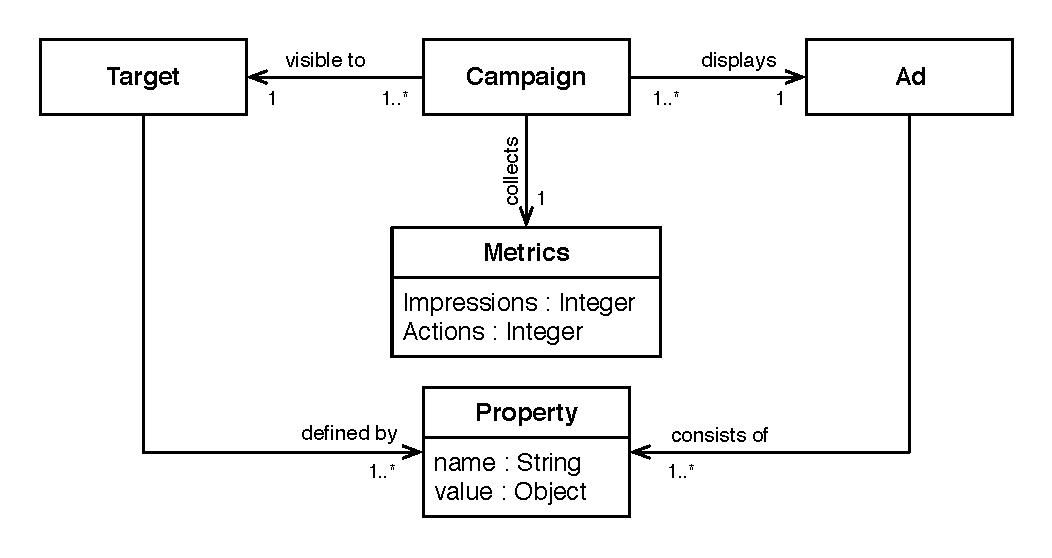
\includegraphics[width=0.9\textwidth]{marketing-uml.eps}
	\caption{UML description of marketing terminology.}
	\label{fig:MarketingTerminology}
\end{figure*}

As the word \emph{user} is typically used to refer to a person interacting with either the web site that is being marketed or the web site on which the advertisement is shown, we will use the word \emph{operator} when discussing a person interacting with the system that is described in this paper to avoid confusion.

\section{Automated marketing}
\begin{figure}[htb] \centering 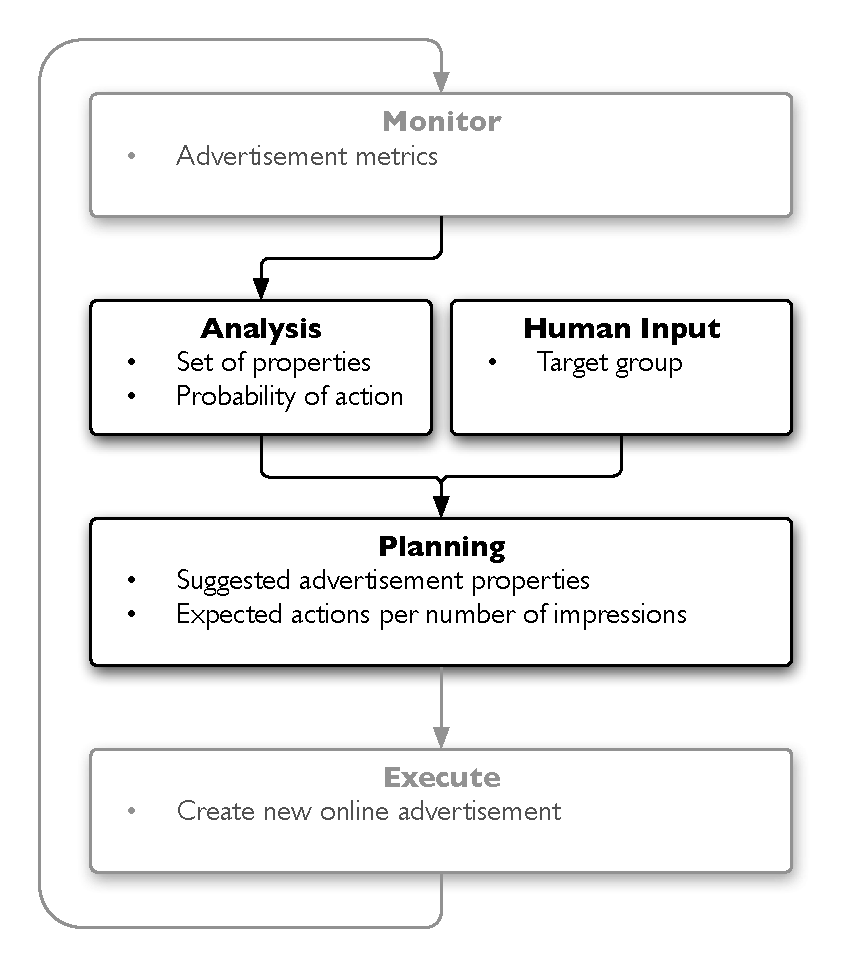
\includegraphics[width=0.5\textwidth]{mape-marketing.eps}
	\caption{Online marketing automation system in control loop}
	\label{fig:MAPEMarketing}
\end{figure}

By merging the fields of automation and online marketing we put the automation terminology in context. Monitoring is the collection of metrics for online advertisement. To optimize these metrics, the gathered information is analyzed and this analysis forms the basis for the planning of future campaigns. Once the plans are completed, the new campaign can be launched, with new metrics being gathered and so on.

Monitoring is commonly automated already, either using custom software or services such as Google Analytics, where as the other parts of the process are performed manually. It is infeasible to fully automate the whole process, due to for example the creative side of advertisement and the complex factors that decide which groups an upcoming campaign should target. There are however certain areas that can be automated and this paper will focus on automated analysis and planning of online marketing campaigns, shown in Figure \ref{fig:MAPEMarketing}.

A system to automate this process requires monitored data as input, which in this context equals historical data of campaigns and their metrics as mentioned previously. This data is then mined to identify subsets of campaign properties that are associated with a probability that an impression of that an ad with these properties leads to an action being taken by the user. Human input is required to specify which target group the next campaign will be aimed at, and based on this the system will generate suggested ad properties that optimize the number of expected actions taken per impression.

\section{Scope}
Using the MAPE framework in Figure \ref{fig:MAPE}, only the analysis and planning tasks are considered part of this paper, where as monitoring and execution are out of scope. The latter two are however relevant in the verification step, but will not be covered as a research topic. In this context, this means for example that the feature of integrating this system with marketing services to automatically add new ads and campaigns will not be a part of the final system.

Furthermore, the data set will likely include attributes whose values are free text and images. Text mining and image recognition are beyond the scope of this project. Instead these attributes will be manually categorized, so that the value space is discrete and finite.

\section{Foundations}
% Knowledge Discovery
A number of high-level descriptions of frameworks for knowledge discovery in databases exist \citep{Fayyad1996, Frawley1992} and they exhibit a number of commonalities. These include the importance of having a knowledgeable human operator guiding the process in terms of supplying domain knowledge to the system formulating the goal of the knowledge discovery; feeding discovered knowledge back into the system; and the identification and application of a discovery method, or more specifically the data mining algorithms.

% Data mining
In data mining, the input to a system can be described using the terms \emph{concepts}, \emph{instances} and \emph{attributes}, where concept is the actual result of the mining, i.e. what we want to be learned; an instance is one single example of data to be mined and can be compared to a row in a database; and attribute is a property of an instance, which in the database analogy is a column \citep{Witten2011}.

Instances are the smallest component of data input to a mining system, but its low-level description of knowledge may not be what is most useful. \citet{Chen1996} give an overview of the field of data mining where they mention the aspect of multi-level data mining, which states that correlations may not commonly exist on the lowest level of granularity, but instead by forming groups of related items. An example given would be that a specific brand of milk does not necessarily imply the purchase of a specific brand of bread, however purchasing milk of any kind may still be correlated to the purchase of bread irrespective of brand.

% Data mining algorithm classes, e.g. classifiers
% TODO: Write stuff

% Decision trees
In a highly influential paper, \citet{Quinlan1986} decribe how decision trees can be created from a training set and how well it handles the problem of unknown attributes values and noisy data. A related paper, \citet{Quinlan1987}, deal with how generated decision trees can be simplified in order to more easily be applied. Four different methods are evaluated, one of which is the reformulation of the tree as a set of production rules. This specific topic is further analyzed in \citet{Quinlan1987b} where such production rules are shown to be more compact and also in many cases improve the classification of unseen data. An added positive effect is that production rules from separate classifications can be merged more efficiently than their original decision trees.

% Case-based reasoning
% TODO: Belongs together with automation
Cased-based reasoning is a methodology that is similair in many ways to the automation framework described previously, but it is more closely related to human cognition. The basic concept as described in \citet{Watson1999} is that in order to solve a new problem, identify (retrieve) existing problems that are similar. Select a solution to one of the retrieved problem and apply it to the current problem (reuse). Adapt (revise) the existing solution to better match the problem at hand, if necessary. Finally, store (retain) the problem and its solution if it was successful.

\chapter{Related works}
\citet{Richardson2007} describe a model for predicting the click-through rates of ads given a set of properties in the context of search engine advertisement. Though it is a relevant subject, the paper is limited to the specific class of search advertising, and is therefore not directly applicable to this paper.

In online advertisement there have been problems of so called click-spam or click-fraud, meaning that the number of clicks on ads is increased in a fraudulent manner, for example using bots. \citet{Dave2012} provides a methodology to measure click-spam in their networks as well as a study of the severity of the problem on different classes of networks. Their results show that established search advertising on for example Google and Bing is fairly accurate in their filtering of click-spam, where as the problem is  greater for contextual and social advertisement, and severe for mobile advertisement. A related paper by \citet{Zhang2011} describes a methodology for advertisers to evaluate the quality of click traffic and use this to assess the difference in quality between bulk traffic vendors and established pay-per-click networks.

Research has also shown that using targeted advertisement is effective given that the ad is not experienced as being obtrusive, though obstrusive ads that are not targeted also increase performance \citep{Goldfarb2011}. This promotes the idea of more effective targeting but may also be important to understand in how the solution presented in this thesis is applied.

Automation in marketing is not a completely novel idea. \citet{Joshi2006} present a technique for automatically finding related keywords for broader targeting of ads by creating a graph of search terms based on the domain knowledge contained in search engines. continuation of that work is that of \citet{Thomaidou2011}, where keywords are also extracted from the landing page to further improve the results. Both approaches are however only relevant for contextual and search engine advertisement.

\chapter{Solution}
The solution has been divided into one section each for the two subtasks identified in the problem description. Analysis covers the problem of creating an appropriate model of the available data that is used in the next stage. Planning, in turn, is the utilization of that model with the purpose of outputting useful information to the operator. Finally, this is followed by the steps taken to evaluate the results.

\section{Analysis}
The first step in the process is analysis, and the first substep is how to deal with the input data. The natural distribution of this data is very uneven because the number of impressions required to receive a click is high. Consider the scenario of a click-through rate (CTR) of 1\%, which means that for every 100 impressions there would on average be one click. The simplest possible classification rule would be a rule that for every instance gives the classification of no click, and this would yield an accuracy of 99\%. Even though this is indeed an impressive number, it is of no use to us since it says nothing about the instances that actually would yield clicks. This is referred to as the problem of imbalanced data sets as described by \citet{Chawla2004}.

One way to deal with this problem is to increase the number of instances that we are interested in (positive instances) or decreasing the number of negative instances in so that the total distribution is even. This is called over-sampling and under- sampling respectively, and will remove the possibility for a classifier to simply disregard the positive instances in the classification \citep{Chawla2004, Japkowicz2002}.

A better alternative is to use the concept of cost modification, i.e. instruct the algorithm that it is more costly to misclassify positive instances as negative instances than vice versa, which has been shown to be as effective as over-sampling but with increased efficiency \citep{Chawla2004, Japkowicz2002} due to the fact that it does not increase the number of instances in the data set.

Once the monitored data has been passed to the system it will be added to the knowledge base. The knowledge base will store all data relating to the marketing campaigns to increase the amount of available data for model generation, described in the next section.

\subsection{Model generation}
% TODO: Argue more for the requirements below
The model is built by any data mining classifier algorithm that adheres to the basic requirements of handling both numerical and categorical values, as well as generating either a decision tree or a set of decision rules, for example the PART algorithm \citep{Frank1998}. The reason for the latter is that the planning step described in the next section requires trees or rules to successfully calculate suggestions.

To increase accuracy, a stratified tenfold cross-validation approach is recommended, which can optionally be repeated ten times to further improve the result with an additional cost in computing time. The validation step calculates the success rate of the classification for each rule or leaf on each pass and average the values on completion.

The monitored data consist of a series of trials, where each trial is either a success or a failure. Each trial is also independent from any other trial. These properties are two of the three geometric properties, and adherence to these mean the data follows a Bernoulli distribution \citep{Milton2002}. Confidence intervals are therefore be calculated using tables for this distribution \citep[chap. 5]{Witten2011} based on the observed success rate \(S\) and the number of instances that matched the rule \(N\). The probability of success (i.e. user action) is \(\rho \pm z\) with confidence \(c\).

As part of the generation of an analysis model, stored estimations may be compared to the monitored data and based on their differences the system updates a number of parameters for the generation algorithm so that future estimates are improved.

\section{Planning}
The goal of the planning step is to identify relevant rules for new campaigns. The definition of relevant is created by the operator, who specifies rules for the target group and inputs them to the system. Based on these conditions of relevancy together with the model created in the analysis step, relevant rules are presented to the user.

Depending on the available training data, there might be targets that are not covered by the generated rule sets. By using rules that are similar to the desired rule, an estimate is created. By creating instances that exactly match the available rules as well as for the input, a distance function is then used to find the instances, and by extension the rules, that most closely resemble the input. Based on these, an estimate is calculated. The estimates may then be stored in the knowledge base to be compared with the observed metrics once the campaign has been run.

Since each rule has a confidence interval of successful classification, multiple rules that are to be merged are weighted based on their accuracy so that rules with high probability of success and a tight confidence interval are preferred. For a single rule, the probability of success, disregarding the confidence interval, is calculated by taking the number of correctly classified instances, \(\rho*N\), divided by the total number of matching instances \(N\).

\section{Evaluation}
The result of the thesis work was verified by applying the results to the problem suggested by Duego in a real-world setting. The suggested advertisement and target groups from the system will be added to their online marketing portfolio which will allow us to analyze the effectiveness of the software. This was done continuously over the course of the development in addition to more traditional software unit and system testing.

The comparison metric to be used is the estimated click rate calculated for each rule set. This number is compared to the actual click rate that the campaign which is created based on the rules receives. Formally, let C be a campaign, \(\hat{M}\) an estimation of C.Metrics, and M the actual metrics of the campaign. If the difference between the values is not statistically significant, i.e. \(|\hat{M} - M| < \epsilon\), the suggestion is considered successful. If the difference is more notable, it might imply that the estimation function requires tuning. The value of \(\epsilon\) must be suitably chosen based on the expected size of the numbers, which may differ between publishers.

\chapter{Discussion}
\section{Risk factors}
Because the output of the system is dependent on historical data, an assumption has been made that older data is still representative of the current state of the marketing. This is definitely not true for campaigns that are adapted for Christmas, Valentine's Day or other special occasions. The assumption is that the amount of such time-dependent data is so small that it will not impact the final results. If however there is reason to believe that this set of data would influence the output, the recommended approach is to remove it from the knowledge base.

% TODO: Move to the actual use of Bernoulli distributions, or removed if not relevant
Another assumption has been that ad impressions are independent of each other. This is in fact a simplification, due to the fact that the same ad may be shown to the same user many times, which might in turn impact how the user looks at the ad because the brand is recognized.

\chapter{Conclusion}
Empty.

\chapter{Proposal}

\section{Research notes}
The Weka Project has defined an input format to be used for their open source data mining software called ARFF (Attribute-Relation File Format) \citep{Garner1995, Witten2011}. This format is used by the Weka software package, but is well-defined and can be used as the input format for custom systems as well. \citet{Witten2011} also describe how to use implementations of Weka in custom software projects as well as how to extend the system with new functionality.

Standard decision trees give a best-effort boolean classification of the input data, however sometimes it might be more appropriate to give the probability that the input belongs to each of the available classes. This can be described using probability estimation trees (PETs). \citet{Provost2003} discuss the problems of estimating these probabilities from ordinary decision trees and goes on to show how to increase the accuracy of the estimates by performing tree pruning more conservately and by applying the Laplace correction. They also show that probability-bagging, meaning the combination of results from multiple classifiers instead of just the one, greatly improves the estimates. The suggested algorithm, called C4.4, is part of a comparative study of PETs by \citet{Chu2011} and is shown to have an impressive accuracy, though other algorithms may still be more appropriate.

\citet{Hahsler2007} presents a package for the R software environment used in statistical computing, which implements a base for transaction databases as well as integration with two of the most common mining algorithms, Apriori and Eclat. One of the useful implementation choices is the implementation of the sparse matrix data structure, which greatly reduces memory load.

\section{Project plan}
The proposed workflow of this thesis is inspired by the agile practices that perhaps most notably have become common in the software development industry. The most important methods that should be applied to this work are iterative project development and frequent ``customer collaboration'', in this case thesis supervisors from both Chalmers University of Technology and Duego Technologies AB.

The project is expected to run for about 20 weeks. By dividing this relatively long period of time into iterations of four weeks, the project will be easier to manage from my point of view as well as provide ample opportunity for the supervisors to have their feedback incorporated.

The initial iterations will most likely require a heavy focus on research and studies of the related fields. The following iterations will include more work on the practical side of the projects. Once the research has progressed to an extent that the problem space as well as the approach of the solution are well defined, more effort can be put into the development of the final application that is to be used by Duego. A preliminary list of milestones is listed below.

\begin{enumerate}
	\item Finish extended proposal (June 19)
	\item Demo a basic prototype of the system (July 9)
	\item Full description and processing of input data (August 14)
	\item Research should be finalized and draft of final paper submitted to supervisors (September 11)
	\item Submit final paper to examinator and working system to Duego (October 9)
\end{enumerate}

\section{Thesis outline}
\begin{itemize}
	\item Abstract (0.5 pages)
 	\item Introduction (5 pages)
 	\item Related works (1 page)
 	\item Solution (10 pages)
 	\begin{itemize}
		\item Analysis step
		\item Planning step
		\item Verification
	\end{itemize}
	\item Discussion (2 page)
	\item Conclusion (1 page)
\end{itemize}

\bibliography{references} % references.bib
\addcontentsline{toc}{chapter}{\numberline{} Bibliography} % For pdf
\setspecialhdr

\newpage

% Appendices
\appendix
\setdefaulthdr
%\input{include/appendix1}
\end{document}